\documentclass{scrartcl}

\usepackage{tabularx} %better tables
\usepackage[table]{xcolor}
\usepackage[utf8]{inputenc}
\usepackage[ngerman]{babel}
\usepackage{hyperref}
\usepackage{tikz}
\usepackage{graphicx}

\begin{document}
	\section*{Realisierungsbericht}
	
	\begin{tabularx}{\textwidth}{| X | X |}
	\hline
	Status & In Arbeit\\
	\hline
	Projektname & DARWIN\\
	\hline
	Projektleiter & Noe Thalheim\\
	\hline
	Auftraggeber & Stefan Schenk\\
	\hline
	Autoren & Yannik Dällenbach, Noe Thalheim\\
	\hline
	\end{tabularx}
	
	\subsection*{Änderungskontrolle}
	\begin{tabularx}{\textwidth}{| X | X | X |}
	\hline
	\rowcolor[gray]{0.9} Version & Datum & Beschreibung\\
	\hline
	1.0 & 12.05.2013 & Init\\
	\hline
	\end{tabularx}
	
	\pagebreak
	%inhaltsverzeichnis
	\tableofcontents
	\pagebreak
	%abschnitt 1
    \section{Zweck des Dokuments}
Zusammenfassung der Ergebnisse der Phase „Realisierung“.
\newpage

	%abschnitt 2
	\section{Technische Detailspezifikation}
\subsection{Innere Struktur}
\subsubsection{Struktur des Systemdesigns}
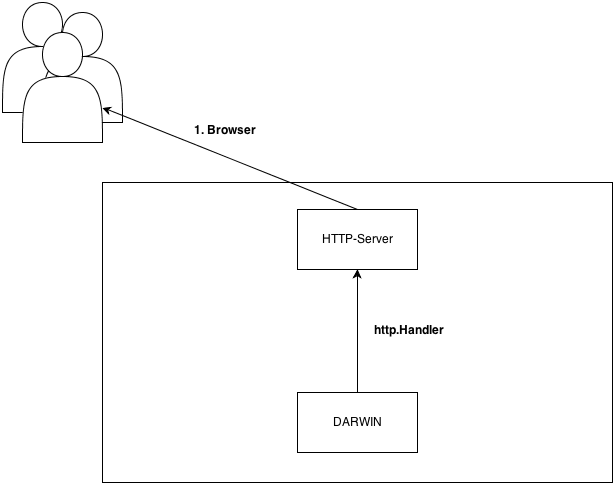
\includegraphics[width=\linewidth]{simplearch.png}
\subsubsection{Beschreibung der Elemente}
Die Architektur von darwin besteht aus 3 Hauptkomponenten.
\subsubsection{Die Spieler}
DARWIN ist ein Multiplayerspiel für bis zu 4 Spieler. Die Spieler können sich via
Netzwerk auf den Server verbinden. Zum Spielen wir ein Browser verwendet.
\subsubsection{Der HTTP-Server}
DARWIN selbst implementiert einen HTTP-Server aus den Standard-Packages von \textbf{go}.
Der HTTP-Server wird für das Hosten der zum Spielen benötigten HTML5-Seiten und
Javascripts verwendet.
\subsubsection{DARWIN (Das Spiel)}
Das Spiel selbst implementiert die allgemeine Spielstruktur welche aus einem Websocket-Server und dem Spiel an sich besteht. Der Websocket-Server implementiert das http.Handler Interface um sich beim HTTP-Server zu registrieren.
\subsection{Schnittstellendefinitionen}
Es werden hauptsächlich zwei Interfaces verwendet.
\subsubsection{1. Browser}
Der Browser stellt die Schnittstelle der Spieler zum Server dar. Diese wurde
mithilfe der Technologien HTML5 und Javascript realisiert.
\subsubsection{http.Handler}
Die http.Handler Schnittstelle wird dazu verwendet eine Methode beim HTTP-Server zu registrieren damit diese per URL-Aufruf ausgeführt wird.
\subsection{Anforderungszuordnung}
%TODO better table an refresh
\begin{tabularx}{\textwidth}{|p{0.7cm}|p{7.0cm}|X|X|}
\hline
Nr. & Anforderung & 1 & 2 \\
\hline
1 & Spielbares Spiel & X & \\
\hline
2 & Lernfähige Gegner & X & X  \\
\hline
3 & Export-Funktion für Gegner & & X  \\
\hline
4 & Bot-Gegen-Bot-Modus & & X    \\
\hline
\end{tabularx}
\newpage

	%abschnitt 3
	\section{Systemdokumentation}
\subsection{Konfigurations-Dokumentation}
Um DARWIN verwenden zu können werden folgende Komponenten benötigt.
\subsubsection{git}
\textbf{git} wird als Versionierungssystem verwendet und um den 
Code von github zu clonen. 
\subsubsection{Go-Compiler Version 1.1}
Mithilfe des Go-Compilers wird der Sourcecode zu einem ausführbaren Binary
kompiliert. Im Allgemeinen wird die Go-Compiler Toolchain zum Auflösen 
der Dependencies von DARWIN und Kompilieren verwendet.
\subsubsection{Umgebungsvariablen}
Um DARWIN verwenden zu können muss das Setup Bash Script(setup.sh) ausgeführt werden.
Dies setzt alle benötigten Umbgebungsvariablen.
\begin{itemize}
    \item PORT
    \item TEMPLATE
\end{itemize}
\textbf{PORT}
\\
Die PORT-Umgebungsvariable spezifiziert an welchem  Port der Webserver sich
bindet.
\\
\textbf{TEMPLATE}
\\
Die TEMPLATE-Umgebungsvariable spezifiziert wo sich die HTML-Templates befinden. 
\subsection{Benutzerhandbuch}
Um das Proof of Concept zu testen sind folgende Punkte zu befolgen:\\
\begin{itemize}
    \item Installieren Sie die Go-Runtime (\url{http://golang.org/})
    \item Downloaden Sie das Proof of Concept (\url{https://github.com/devNil/darwin}) 
    \item Starten Sie das Proof of Concept mit dem Befehl \textbf{go run main.go}
\end{itemize}

\subsection{Supporthandbuch}
Für die technisch versierten Benutzer besteht die Möglichkeit Parameter des Proof of Concet zu ändern, diese befinden sich in der Datei game.go. \\

    %abschnitt 4
	\section{Systemtest}
\subsection{Testspezifikation}
\subsubsection{Testverfahren}
\subsubsection{Test-Szenario}
\subsubsection{Testfälle}
\subsection{Testprotokoll}
\subsubsection{Testobjekt}
\subsubsection{Testresultate}
\subsubsection{Testauswertung}

    %abschnitt 5
	\input{4_1_realisierungsbericht5}
%	\usetikzlibrary{arrows,positioning}
	
\section{Planung und Organisation}
	
\subsection{Projektorganisation}
An dem Projekt werden folgende Personen mitarbeiten:
\\\\
\begin{tikzpicture}[node distance=1cm, auto]  
\tikzset{
	    mynode/.style={rectangle,align=left,draw=black, top color=white, bottom color=white!50,very thick, inner sep=1em, minimum size=3em, text centered},
	    myarrow/.style={->, >=latex', shorten >=1pt, thick},
	    mylabel/.style={text width=7em, text centered} 
	}  
	\node[mynode] (auftraggeber) {\textbf{Auftraggeber}\\Stefan Schenk};  
	\node[mynode, below=1cm of auftraggeber] (projektleiter) {\textbf{Projektleiter}\\Noe Thalheim};  
	\node[mynode, right=of projektleiter] (projektmitarbeiter1) {\textbf{Projektmitarbeiter}\\Yannik Dällenbach};


	\draw[myarrow] [<->] (auftraggeber.south) -- (projektleiter.north);	
	\draw[myarrow] [-] (projektleiter.east) -- (projektmitarbeiter1.west);

	\end{tikzpicture} 
	\medskip

	Die Aufgabenverteilung wird das ganze Projekt gleich bleiben.
	
	\subsection{Termine}
	
	Für unser Projekt sind folgende Termine von Wichtigkeit:
	\begin{description}
		\item[] Starttermin: 05.02.2013
		\item[] Endtermin: 04.06.2013
	\end{description}
	Daraus ergibt sich für unser Projekt folgender Terminplan:
	\\ \\
	\tiny{
	\begin{tabular}{| p{2cm} | p{1cm} | p{1cm} | p{1cm} | p{1cm} | p{1cm} | p{1cm} |}
	\hline
	\rowcolor[gray]{0.9}  & 12.02.13 - 19.02.13 & 19.02.13 - 05.03.13 & 5.03.13 - 19.03.13 & 19.03.13 - 07.05.13 & 7.05.13 - 21.05.13 & 21.05.13 - 04.06.13 \\
	\hline
	Initialisierung & \cellcolor{yellow} & & & & & \\
	\hline
	Voranalyse & &  \cellcolor{yellow}& & & & \\
	\hline
	Konzept & & &  \cellcolor{yellow}& & & \\
	\hline
	Realisierung & & & &  \cellcolor{yellow}& & \\
	\hline
	Einführung & & & & & \cellcolor{yellow}& \\
	\hline
	Abschluss & & & & &  &\cellcolor{yellow} \\
	\hline
	\end{tabular}	
	}
	\small{
	\\ \\
	Unser Aufgabenplanung werden wir folgendermassen gestalten: 

	\begin{figure}[htb]

	\centering

	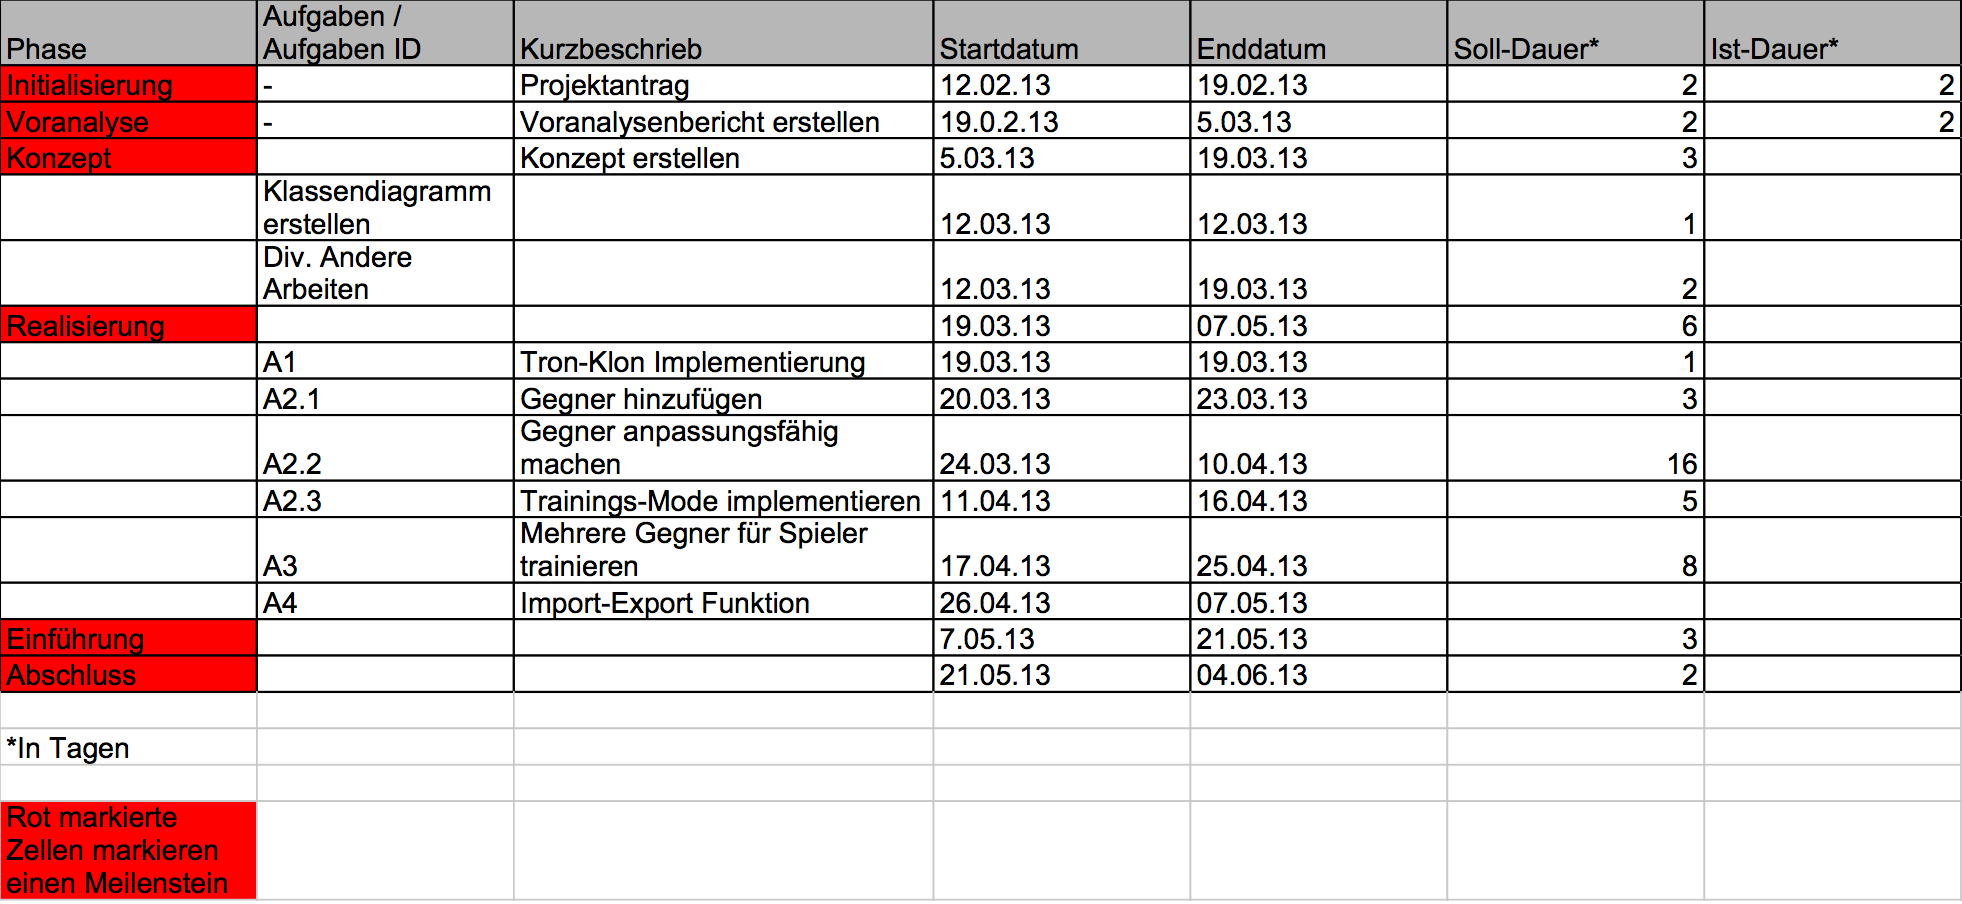
\includegraphics[width=\textwidth]{plan.png}

	\caption{Momentane Aufgabenplanung}

	\end{figure}

	\subsection{Prioritäten}
	Unsere Prioritäten für dieses Projekt sind das Verstehen und Implementieren von Evolutionären Algorithmen und somit das Selbststudium in diesen Gebieten. Zudem ist es uns wichtig durch dieses Projekt Erfahrungen im Zusammenhang mit der Programmierung in Objective-C sammeln zu können. 
}
%	\section{Wirtschaftlichkeit}
	DARWIN soll in einem Proof of Concept aufzeigen wie sich Evolutionäre Algorithmen bewähren, Gegner in einem Spiel dem Spieler anzupassen. Das Projekt hat keinen wirtschaftlichen Aspekt im allgemeinen Sinne, könnte jedoch als Grundlage für ein späteres Projekt dienen.
%	\section{Konsequenzen und Risiken}
\subsection{Risikobeurteilung}
Da es sich bei unserem Projekt um Themen handelt, bei denen keines der Projektmitglieder auf grosse Erfahrung bauen kann ist das grösste Risiko, dass wir Probleme mit der Realisierung der Evolutionären Algorithmen haben werden und somit unser Proof of Concept nicht fertigstellen könnten. Den Tron-Klon auf welchem unser Proof of Concept basiert, können wir hingegen ohne grossen Aufwand realisieren.

\subsection{Ausweichmöglichkeiten}
Falls es tatsächlich soweit kommen sollte, dass es uns nicht möglich ist die von uns erwähnten Evolutionären Algorithmen zu implementieren werden wir uns Hilfe von aussenstehenden organisieren oder die Evolutionären Algorithmen weglassen und uns auf den Tron-Klon konzentrieren. 
%	\pagebreak
\section{Antrag}
	Wir beantragen die Genehmigung des vorliegenden Voranalyseberichts und die Freigabe für die Phase Konzept durch den Auftraggeber.
	\\ \\ \\
	Noe Thaleim:
	\\ \\
	\parbox{4cm}{\hrule
	\strut \centering\footnotesize Ort, Datum} \hfill\parbox{4cm}{\hrule
	\strut \centering\footnotesize Unterschrifft}
	\\ \\ \\
	Yannik Dällenbach:
	\\ \\
	\parbox{4cm}{\hrule
	\strut \centering\footnotesize Ort, Datum} \hfill\parbox{4cm}{\hrule
	\strut \centering\footnotesize Unterschrifft}
	\\ \\ \\
	Für den Auftraggeber:
	\\ \\
	\parbox{4cm}{\hrule
	\strut \centering\footnotesize Ort, Datum} \hfill\parbox{4cm}{\hrule
	\strut \centering\footnotesize Unterschrifft}
\end{document}
